\section{Payload \& Handler}

\begin{center}
    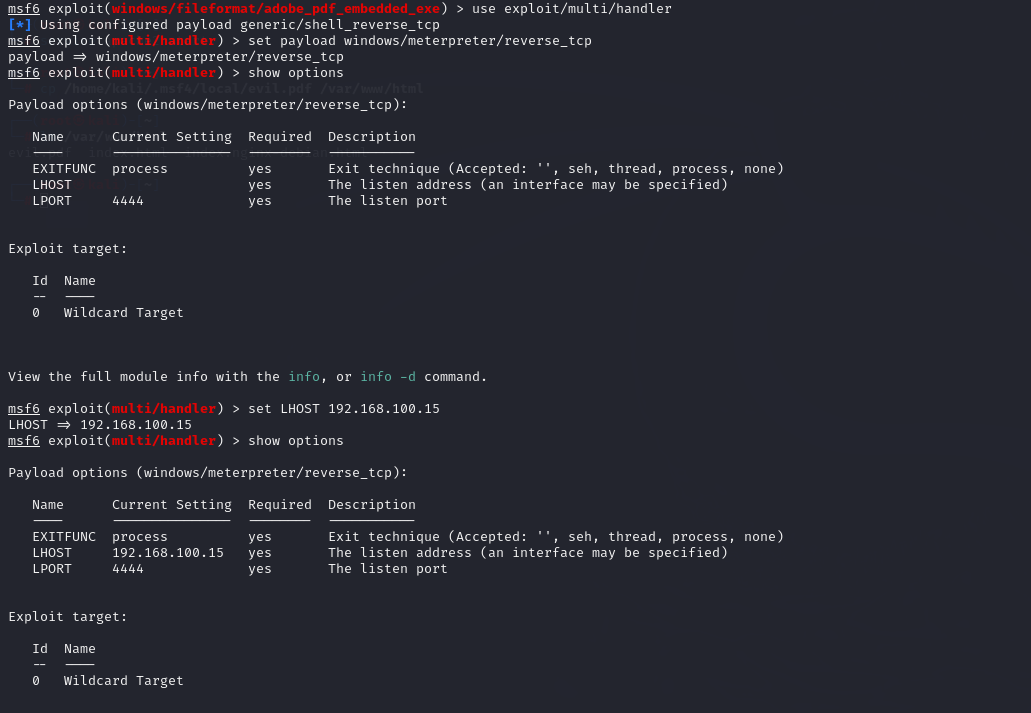
\includegraphics[width=0.8\textwidth]{Question/SC/13_14_15-.PNG}
\end{center}

\vspace{0.15cm}

\begin{center}
    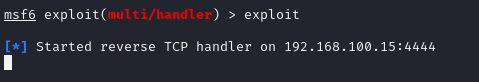
\includegraphics[width=0.6\textwidth]{Question/SC/16.PNG}
\end{center}

\vspace{0.15cm}

\begin{center}
    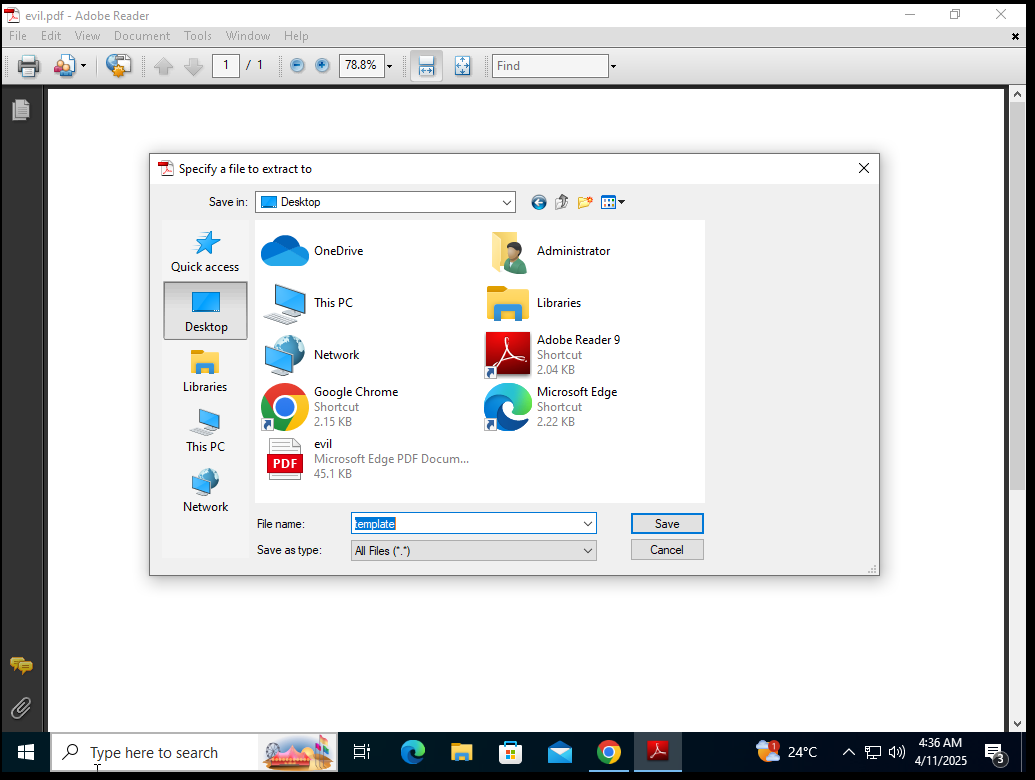
\includegraphics[width=0.6\textwidth]{Question/SC/17.PNG}
\end{center}

\vspace{0.15cm}
\begin{center}
    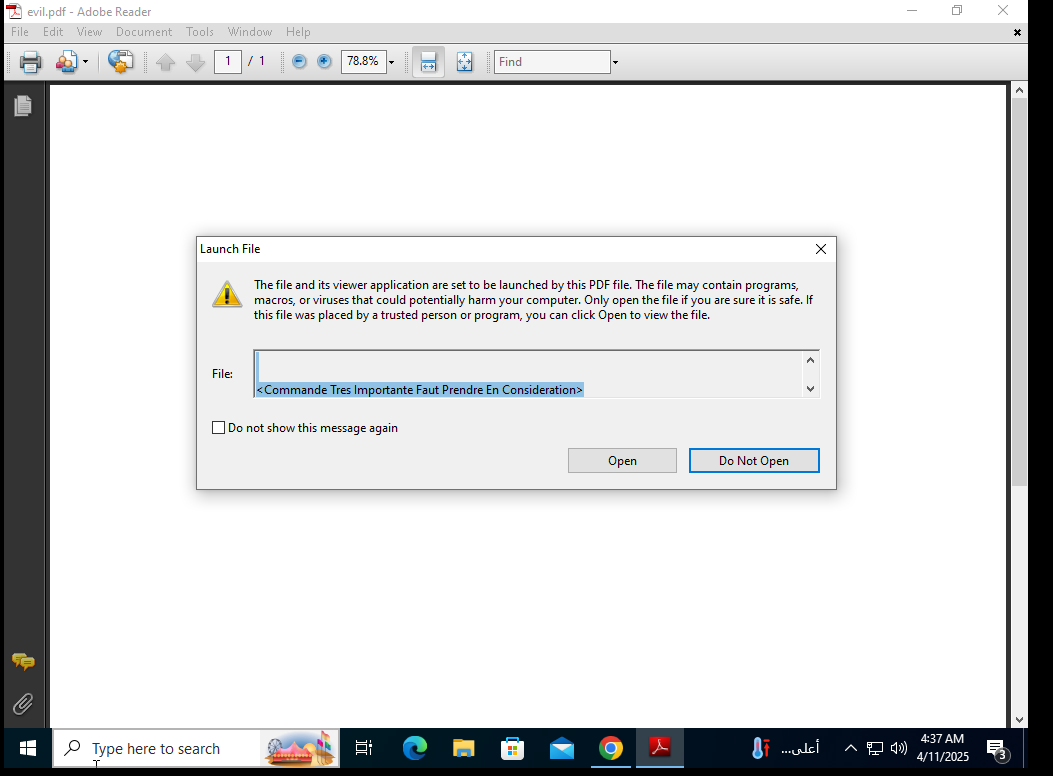
\includegraphics[width=0.6\textwidth]{Question/SC/18.PNG}
\end{center}


\vspace{0.35cm}


\begin{prettyBox}{Définitions Des Termes}{myblue}
    \begin{itemize}
        \item \textbf{Handler} : programme exécuté sur la machine de l'attaquant, qui se met en écoute afin d'attendre une connexion provenant de la victime lorsqu'elle exécute le payload (par exemple, en ouvrant un lien ou un fichier malveillant).
        \item \textbf{Payload} : programme malveillant exécuté sur la machine de la victime suite à une action spécifique réalisée par celle-ci.
        \item \textbf{Reverse Shell} : mécanisme permettant à l'attaquant d'exécuter des commandes shell sur la machine de la victime depuis sa propre machine, en utilisant une connexion TCP inverse initiée par la victime.
        \item \textbf{Message affiché} : message qui apparaît sur la machine de la victime, identique à celui configuré précédemment via la commande \texttt{set LAUNCH\_MESSAGE}.
    \end{itemize}
\end{prettyBox}

